%%%%%%%%%%%%%%%%%%%%%%%%%%%%%%%%%%%%%%%%%%%%%%%%%%%%%%%%%%%%%%%%%%%%%%%%%%%%%%%
% Appendix C - Sterile Cranial Window Surgical Preparation
%%%%%%%%%%%%%%%%%%%%%%%%%%%%%%%%%%%%%%%%%%%%%%%%%%%%%%%%%%%%%%%%%%%%%%%%%%%%%%%

\chapter{Sterile Cranial Window Surgical Preparation} \label{app:cranial_window}

While the optical imaging techniques described in this dissertation are non-contact, a chronic cranial window implantation is required to obtain optical access to brain tissue. This appendix details the craniotomy procedure and maintenance protocol utilized for chronic \textit{in vivo} awake imaging in mice. All animal protocols were approved by the Institutional Animal Care and Use Committee at The University of Texas at Austin.


%%%%%%%%%%%%%%%%%%%%%%%%%%%%%%%%%%%%%%%%%%%%%%%%%%%%%%%%%%%%%%%%%%%%%%%%%%%%%%%
% Section B.1 - Implantation of Cranial Window
%%%%%%%%%%%%%%%%%%%%%%%%%%%%%%%%%%%%%%%%%%%%%%%%%%%%%%%%%%%%%%%%%%%%%%%%%%%%%%%
\section{Implantation of Cranial Window}

Mice (CD-1, male, 25-30 g, Charles River) were anesthetized with medical air vaporized isoflurane (2.0\%) via nose-cone inhalation. Body temperature was maintained at 37 $^\circ$C with a feedback heating pad (DC Temperature Controller, FHC). Arterial oxygen saturation, heart rate, and breath rate were monitored via pulse oximetry (MouseOx, Starr Life Sciences). After induction, mice were placed supine in a head-fixed stereotaxic frame (Narishige Scientific Instrument Lab) and administered carprofen (5 mg/kg, subcutaneous) for anti-inflammation and dexamethasone (2 mg/kg, intramuscular) to reduce the severity of cerebral edema following removal of the skull. Surgical instruments and artificial cerebrospinal fluid (ACSF, buffered pH 7.4) used during the craniotomy procedure were sterilized in an autoclave.

% Figure - Cranial Window Location
\begin{figure}
    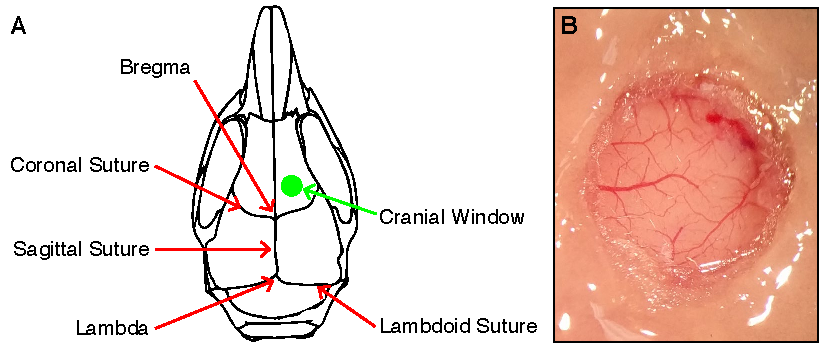
\includegraphics{figures/appendix_c/cranialwindow.pdf}
    \caption[Location of the cranial window on the mouse skull]{
        \label{fig:cranialwindow}
        Location of the cranial window relative to bregma. Skull illustratrion adapted from \cite{Cook:1965wb}.
    }
\end{figure}

The scalp was shaved and resected to expose skull between the bregma and lambda cranial coordinates. A thin layer of cyanoacrylate (Vetbond Tissue Adhesive, 3M) was applied to the exposed skull to facilitate the adhesion of dental cement during a later step. A 2-3 mm diameter portion of the skull over the frontoparietal cortex was removed while leaving the dura intact using a dental drill (0.8 mm burr, Ideal Microdrill, Fine Science Tools) with regular ACSF perfusion to prevent overheating. A 5 mm round cover glass (\#1.5, World Precision Instruments) was placed over the exposed brain and a dental cement mixture was deposited along the perimeter while applying gentle pressure to the cover glass. This process bonded the cover glass to the surrounding skull to create a sterile, air-tight seal around the craniotomy and allowed for restoration of intracranial pressure. A second layer of cyanoacrylate was applied over the dental cement to further seal the cranial window. The medial and anterior edges of the window were approximately 2 mm rostral from bregma and 0.5 mm lateral from the sagittal suture (Figure \ref{fig:cranialwindow}). Animals were allowed to recover from anesthesia and monitored for cranial window integrity and normal behavior for at least two weeks prior to imaging. Additional carprofen injections (5 mg/kg) were administered subcutaneously two, four, and seven days post-surgery to relieve inflammation from the procedure.


%%%%%%%%%%%%%%%%%%%%%%%%%%%%%%%%%%%%%%%%%%%%%%%%%%%%%%%%%%%%%%%%%%%%%%%%%%%%%%%
% Section B.2 - Headbar Attachment
%%%%%%%%%%%%%%%%%%%%%%%%%%%%%%%%%%%%%%%%%%%%%%%%%%%%%%%%%%%%%%%%%%%%%%%%%%%%%%%
\section{Headbar Attachment} \label{app:headbar_attachment}

Animals designated for awake imaging underwent an additional procedure during the application of dental cement to permanently attach a metal headbar used for head fixation. The circular cutout in the headbar was aligned with the cranial window and rotated laterally until parallel with the cover glass. This ensured that the cranial window would be perpendicular to the imaging system's optical axis when the animal was restrained in the awake imaging setup. Dental cement was applied around the headbar to permanently attach it to the animal's skull.


%%%%%%%%%%%%%%%%%%%%%%%%%%%%%%%%%%%%%%%%%%%%%%%%%%%%%%%%%%%%%%%%%%%%%%%%%%%%%%%
% Section B.3 - Chronic Animal Maintenance
%%%%%%%%%%%%%%%%%%%%%%%%%%%%%%%%%%%%%%%%%%%%%%%%%%%%%%%%%%%%%%%%%%%%%%%%%%%%%%%
\section{Chronic Animal Maintenance}

Animals were checked daily to monitor both behavior and the integrity of the cranial window by veterinary staff at the University of Texas at Austin Animal Research Center (ARC). Animals were housed in climate-controlled rooms with timed lighting (12-hour light/dark cycles) to maintain a comfortable living environment and given food and water \textit{ad libitum}. Social housing with multiple animals reduced the risk of overeating commonly seen when solo housing animals. This minimized possible growth in the animal's size and helped maintain the integrity of the cranial window. Any aggression resulted in the removal of the aggressor into a separate cage.

After several weeks of recovery, animals were used for both acute and chronic imaging experiments. Cranial windows were lightly cleaned prior to each imaging session using a cotton swab and 70\% ethanol (v/v). If necessary, a topical application of mineral oil was used to improve image quality by index matching. Any discoloration on or around the cranial window was documented and monitored for possible infection. Any cracks in or breaking of the cranial window were also documented and resulted in the immediate euthanasia of the animal.


%%%%%%%%%%%%%%%%%%%%%%%%%%%%%%%%%%%%%%%%%%%%%%%%%%%%%%%%%%%%%%%%%%%%%%%%%%%%%%%
% END Appendix B
%%%%%%%%%%%%%%%%%%%%%%%%%%%%%%%%%%%%%%%%%%%%%%%%%%%%%%%%%%%%%%%%%%%%%%%%%%%%%%%
